% Options for packages loaded elsewhere
\PassOptionsToPackage{unicode}{hyperref}
\PassOptionsToPackage{hyphens}{url}
\PassOptionsToPackage{dvipsnames,svgnames,x11names}{xcolor}
%
\documentclass[
  authoryear,
  preprint,
  3p]{elsarticle}

\usepackage{amsmath,amssymb}
\usepackage{lmodern}
\usepackage{iftex}
\ifPDFTeX
  \usepackage[T1]{fontenc}
  \usepackage[utf8]{inputenc}
  \usepackage{textcomp} % provide euro and other symbols
\else % if luatex or xetex
  \usepackage{unicode-math}
  \defaultfontfeatures{Scale=MatchLowercase}
  \defaultfontfeatures[\rmfamily]{Ligatures=TeX,Scale=1}
\fi
% Use upquote if available, for straight quotes in verbatim environments
\IfFileExists{upquote.sty}{\usepackage{upquote}}{}
\IfFileExists{microtype.sty}{% use microtype if available
  \usepackage[]{microtype}
  \UseMicrotypeSet[protrusion]{basicmath} % disable protrusion for tt fonts
}{}
\makeatletter
\@ifundefined{KOMAClassName}{% if non-KOMA class
  \IfFileExists{parskip.sty}{%
    \usepackage{parskip}
  }{% else
    \setlength{\parindent}{0pt}
    \setlength{\parskip}{6pt plus 2pt minus 1pt}}
}{% if KOMA class
  \KOMAoptions{parskip=half}}
\makeatother
\usepackage{xcolor}
\setlength{\emergencystretch}{3em} % prevent overfull lines
\setcounter{secnumdepth}{5}
% Make \paragraph and \subparagraph free-standing
\ifx\paragraph\undefined\else
  \let\oldparagraph\paragraph
  \renewcommand{\paragraph}[1]{\oldparagraph{#1}\mbox{}}
\fi
\ifx\subparagraph\undefined\else
  \let\oldsubparagraph\subparagraph
  \renewcommand{\subparagraph}[1]{\oldsubparagraph{#1}\mbox{}}
\fi


\providecommand{\tightlist}{%
  \setlength{\itemsep}{0pt}\setlength{\parskip}{0pt}}\usepackage{longtable,booktabs,array}
\usepackage{calc} % for calculating minipage widths
% Correct order of tables after \paragraph or \subparagraph
\usepackage{etoolbox}
\makeatletter
\patchcmd\longtable{\par}{\if@noskipsec\mbox{}\fi\par}{}{}
\makeatother
% Allow footnotes in longtable head/foot
\IfFileExists{footnotehyper.sty}{\usepackage{footnotehyper}}{\usepackage{footnote}}
\makesavenoteenv{longtable}
\usepackage{graphicx}
\makeatletter
\def\maxwidth{\ifdim\Gin@nat@width>\linewidth\linewidth\else\Gin@nat@width\fi}
\def\maxheight{\ifdim\Gin@nat@height>\textheight\textheight\else\Gin@nat@height\fi}
\makeatother
% Scale images if necessary, so that they will not overflow the page
% margins by default, and it is still possible to overwrite the defaults
% using explicit options in \includegraphics[width, height, ...]{}
\setkeys{Gin}{width=\maxwidth,height=\maxheight,keepaspectratio}
% Set default figure placement to htbp
\makeatletter
\def\fps@figure{htbp}
\makeatother

\usepackage{booktabs}
\usepackage{longtable}
\usepackage{array}
\usepackage{multirow}
\usepackage{wrapfig}
\usepackage{float}
\usepackage{colortbl}
\usepackage{pdflscape}
\usepackage{tabu}
\usepackage{threeparttable}
\usepackage{threeparttablex}
\usepackage[normalem]{ulem}
\usepackage{makecell}
\usepackage{xcolor}
\usepackage{todonotes,mathtools,bm,amsmath,mathpazo}
\mathtoolsset{showonlyrefs}
\setlength{\parindent}{0cm}
\makeatletter
\makeatother
\makeatletter
\makeatother
\makeatletter
\@ifpackageloaded{caption}{}{\usepackage{caption}}
\AtBeginDocument{%
\ifdefined\contentsname
  \renewcommand*\contentsname{Table of contents}
\else
  \newcommand\contentsname{Table of contents}
\fi
\ifdefined\listfigurename
  \renewcommand*\listfigurename{List of Figures}
\else
  \newcommand\listfigurename{List of Figures}
\fi
\ifdefined\listtablename
  \renewcommand*\listtablename{List of Tables}
\else
  \newcommand\listtablename{List of Tables}
\fi
\ifdefined\figurename
  \renewcommand*\figurename{Figure}
\else
  \newcommand\figurename{Figure}
\fi
\ifdefined\tablename
  \renewcommand*\tablename{Table}
\else
  \newcommand\tablename{Table}
\fi
}
\@ifpackageloaded{float}{}{\usepackage{float}}
\floatstyle{ruled}
\@ifundefined{c@chapter}{\newfloat{codelisting}{h}{lop}}{\newfloat{codelisting}{h}{lop}[chapter]}
\floatname{codelisting}{Listing}
\newcommand*\listoflistings{\listof{codelisting}{List of Listings}}
\makeatother
\makeatletter
\@ifpackageloaded{caption}{}{\usepackage{caption}}
\@ifpackageloaded{subcaption}{}{\usepackage{subcaption}}
\makeatother
\makeatletter
\@ifpackageloaded{tcolorbox}{}{\usepackage[many]{tcolorbox}}
\makeatother
\makeatletter
\@ifundefined{shadecolor}{\definecolor{shadecolor}{rgb}{.97, .97, .97}}
\makeatother
\makeatletter
\makeatother
\journal{Journal of}
\ifLuaTeX
  \usepackage{selnolig}  % disable illegal ligatures
\fi
\usepackage[]{natbib}
\bibliographystyle{elsarticle-harv}
\IfFileExists{bookmark.sty}{\usepackage{bookmark}}{\usepackage{hyperref}}
\IfFileExists{xurl.sty}{\usepackage{xurl}}{} % add URL line breaks if available
\urlstyle{same} % disable monospaced font for URLs
\hypersetup{
  pdftitle={Pharmaceutical Supply Chain Forecasting by using Machine Learning in Ethiopian Pharmaceutical Supply Services},
  pdfauthor={Arebu Issa Bilal; Arebu Issa Bilal; Bahman Rostami-Tabar; Umit Sezer Bititci; Teferi Gedif Fenta},
  pdfkeywords={Pharmaceutical Demand Forecasting, Ethiopian
Pharmaceutical Supply Services, ARIMA Model, Forecasting
Variables, Forecast Accuracy},
  colorlinks=true,
  linkcolor={blue},
  filecolor={Maroon},
  citecolor={Blue},
  urlcolor={Blue},
  pdfcreator={LaTeX via pandoc}}


\begin{document}

\begin{frontmatter}
\title{Pharmaceutical Supply Chain Forecasting by using Machine Learning
in Ethiopian Pharmaceutical Supply Services}
\author[1]{Arebu Issa Bilal%
\corref{cor1}%
}
 \ead{arebu.issa@aau.edu.et} 
\author[]{Arebu Issa Bilal%
%
}
 \ead{arebu.issa@aau.edu.et} 
\author[2]{Bahman Rostami-Tabar%
%
}
 \ead{rostami-tabarb@cardiff.ac.uk} 
\author[3]{Umit Sezer Bititci%
%
}
 \ead{U.S.Bititci@hw.ac.uk} 
\author[1]{Teferi Gedif Fenta%
%
}
 \ead{tgedif@gmail.com} 

\affiliation[1]{organization={Addis Ababa University, Department of
Pharmaceutics and Social Pharmacy at School of
Pharmacy},country={Ethiopia},countrysep={,},postcode={9086},postcodesep={}}
\affiliation[2]{organization={University, Cardiff Business
School},country={UK},countrysep={,},postcode={CF5},postcodesep={}}
\affiliation[3]{organization={University, Edinburgh Business
School},country={UK},countrysep={,},postcode={EH14 4AS},postcodesep={}}

\cortext[cor1]{Corresponding author}





        
\begin{abstract}
This study delves into the realm of pharmaceutical demand forecasting
within the Ethiopian Pharmaceuticals Supply Services(EPSS) context. It
encompasses a comprehensive analysis of 37 key pharmaceutical
products,assessing their forecast accuracy across variation models. The
initial assessment reveals that the Autoregressive Integrated Moving
Average (ARIMA) model emerges as a frotrunner, boasting a Root Mean
Squared Error (RMSSE) value of 0.850. ARIMA's prowess in capturing
complex demand patterns suggests its suitability for pharmaceutical
sales forecasting in the EPSS landscape. To argument forecasting
accuarcy, predictor varaibles such as physical count, budget release and
closure by the goverment, the impact of COVID-19, and promotional
campaigns were incorpoarted. Remarkably, the ARIMA model mantainsits
superiority even in the presences of these external factors, reiterating
its roustness. Delving further into individual pharmaceutical products,
ARIMA with predictors demonstrates exceptional performance for a
substantial portion (32.43\%) of the products, including Amoxicillin
500mg capsule, Anti RhD, Artehmether + Lumefantrine, and others.
Conversely,alternative models like naive, mean, and regression methods
showcase strengths for different pharmaceutical categories, underscoring
the importance of tailoring forecasting approaches to product-specific
dynamics. While this study significantly advances the discourse on
pharmaceutical demand forecasting, limitations stemming from data
quality and external variables underscore the intricacies of the
forecasting landscape. In conclusion, it advocates the integration of
the ARIMA model with predictor variables as a strategic approach for
refining pharmaceutical demand forecasting within EPSS. It also
encourages further exploration of advanced forecasting techniques and
ongoing refinement to bolster supply chain efficiency and ensure
consistent pharmaceutical availability. Capacity building through staff
training and replication of the study in diverse healthcare settings are
recommended steps toward resilient and efficient pharmaceutical supply
chains.These findings hold promise for fostering supply chains that are
adaptable, responsive, and capable of ensuring the continuous
availability of essential pharmaceuticals in Ethiopia.
\end{abstract}





\begin{keyword}
    Pharmaceutical Demand Forecasting \sep Ethiopian Pharmaceutical
Supply Services \sep ARIMA Model \sep Forecasting Variables \sep 
    Forecast Accuracy
\end{keyword}
\end{frontmatter}
    \ifdefined\Shaded\renewenvironment{Shaded}{\begin{tcolorbox}[borderline west={3pt}{0pt}{shadecolor}, interior hidden, breakable, enhanced, frame hidden, sharp corners, boxrule=0pt]}{\end{tcolorbox}}\fi

\hypertarget{sec-intro}{%
\section{Introduction}\label{sec-intro}}

Universal access essential medicines is a cornerstone of effective
healthcare systems, yet ensuring equitable availability of these vital
medications remains an urgent global
challenge\citep{quick2003essential, world2004annual}. Across continents,
especially in Africa and Asia, many nations grapple with restricted
access due to factors like unaffordability and suboptimal supply chain
management \citep{world2004medicines}. A survey conducted across eight
sub-Saharan African countries indicated that there were unacceptably low
availability of essential medicines.The mean availability of 12 priority
essential medicines for women ranged from 22\% to 40\% and from 28\% to
57\% for children \citep{droti2019poor}. However, the issue of drug
shortages extends beyond developing countries, with instances reported
in the United States and Europe, adversely impacting healthcare systems
and compromising patient care quality
\citetext{\citealp[\citet{kaakeh2011impact}]{fox2003managing}; \citealp{johnson2011drug}; \citealp{huys2013european}; \citealp{le2011prevalence}}.

The consequences of drug shortages are felt both financially within the
healthcare sector and in terms of the quality of patient care
\citep{alspach2012drug, kaakeh2011impact, kaakeh2011impact, baumer2004national}.The
consequences extend across patients, providers, healthcare institutions,
and research programs. Patients face delays or cancellations of
treatments, substandard care due to the unavailability of optimal
therapies, and increased costs in a secondary ``grey market.''
Compromised patient safety, complications, prolonged hospital stays, and
even deaths have been reported {[}\citet{alspach2012drug};{]}.Addressing
these shortages is crucial to preserving the quality of patient care and
ensuring the effectiveness of healthcare delivery. Thus, a smoothly
operating pharmaceutical supply chain is essential to ensure timely
access to essential medicines, making accurate demand forecasting an
indispensable component.

An efficient pharmaceutical supply chain is vital for timely access to
essential health commodities. One of the most crucial components of such
a supply chain is a well-defined demand forecasting process. Forecasting
accurately the future demand for essential medicines provides valuable
insights for anticipating future healthcare requirements including
procurement and replenishment of
inventory\citep{subramanian2021effective}. Despite the significance of
forecasting for supply chain management, pharmaceutical product
forecasting remains a complex endeavor influenced by a multitude of
factors. Key considerations include the availability of data, the
specific position within the supply chain, and the nuanced understanding
of contributing elements. The position within the supply chain
introduces unique challenges and dynamics, requiring tailored
forecasting approaches. Additionally, a nuanced understanding of
contributing elements involves grasping intricate factors that impact
forecasting accuracy, such as market trends, regulatory changes, and
external influences. Schneider, Wilson, and Rosenbeck (2010) and Hyndman
and Athanasopoulos (2018) highlight the intricate nature of
pharmaceutical forecasting, emphasizing the need for a comprehensive
approach that incorporates these multifaceted aspects to enhance supply
chain management
effectiveness\citep{schneider2010pharmaceutical, hyndman2018forecasting}.

The Ethiopian pharmaceutical sector's distinct characteristics, marked
by a diverse array of medicines and unique data challenges stemming from
service delivery points, staff capacity limitations, communication
hurdles, prolonged procurement and distribution lead times, poor
forecast accuracy, and policy intricacies, necessitates tailored
forecasting strategies that cater to the nation's specific context
\citep{boche2022procurement}. In this context, a comprehensive
exploration of effective forecasting models that align with Ethiopia's
pharmaceutical landscape is paramount to mitigating stock outs and
enhancing healthcare delivery. The implications of pharmaceutical demand
forecasting extend beyond financial considerations to societal
well-being \citep{rostami2022forecasting}. In Ethiopia, a country
undergoing demographic and healthcare evolution, precise demand
forecasting assumes immense importance for resource allocation, supply
chain optimization, and policy formulation. With mounting interest in
refining demand forecasting in Ethiopia's pharmaceutical sector, this
study seeks to contribute to existing knowledge by investigating and
recommending proficient demand forecasting methods. Our investigation
centers on the application of mean, naive, exponential smoothing,
regression, and ARIMA models to bolster forecast accuracy and
effectiveness. This paper aims to forecast the demand for selected
pharmaceuticals in EPSS over the next 12 months by utilizing various
forecasting models and integrating predictors. The integration of
predictors with the models will be examined to determine whether they
enhance the forecasting accuracy. These predictors are derived from a
historical analysis of events in Ethiopia over the last 5 years that
have impacted pharmaceutical sales in EPSS. These events include
COVID-19, conflicts in the country, disease campaigns, budget closures,
budget releases, and physical inventory, all of which, in varying
degrees, influence the demand for pharmaceuticals in Ethiopia.

The current paper offers the following contributions we aim at
forecasting pharmaceutical sales over a 12-month period these models aim
to enhance the accuracy and reliability of demand predictions within the
context of EPSS. Moreover an essential contribution lies in the
identification of key factors influencing pharmaceutical sales. The
study develops a model that effectively incorporates these driving
factors, providing a more nuanced and comprehensive approach to demand
prediction. We generate forecasts and evaluate model performance using
the Root Mean Squared Error (RMSE), Root Mean Squared Scaled Error
(RMSSE) and Mean Absolute Error (MAE), Mean Absolute Scaled Error
(MASE), Crips and Winkler are used to assess probabilistic forecast
accuracy. \#how you know the forecasting accutacy problem and provide
eveidence about the forecasting problems \# most forecast focus on point
forecast and we want to focus on probablistic forecast \# i will write
the contribution of the reearch rather than these objectives

This research is guided by several objectives:

\begin{enumerate}
\def\labelenumi{\arabic{enumi}.}
\tightlist
\item
  Evaluate the robustness of various forecasting models for
  pharmaceutical demand prediction within EPSS.
\item
  Identify pharmaceuticals that exhibit superior forecast accuracy under
  specific models.
\item
  Assess the performance of forecast accuracy metrics to gauge the
  efficacy of selected models.
\item
  Test the incorporation of diverse predictors affecting forecasts and
  evaluate resulting forecasting accuracy. In pursuing these objectives,
  this study endeavors to elevate the precision and reliability of
  pharmaceutical demand forecasting, thereby contributing to optimized
  supply chain management and enhanced healthcare outcomes in Ethiopia.
\end{enumerate}

\hypertarget{sec-lit}{%
\section{Research background}\label{sec-lit}}

Precise sales prediction is an essential and inexpensive way for each
company to augment their profits, decrease their costs, and achieve
greater flexibility to changes. In other words, exact sales forecasting
is utilized for capturing the tradeoff between customer demand
satisfaction and inventory costs \citep{gupta2000mid}. Especially, for
the pharmaceutical industry, successful sales forecasting systems can be
very beneficial, due to the short shelf-life of many pharmaceutical
products and the importance of the product quality which is closely
related to the human health \citep{doganis2006time}.There are many
decisions that depend on the quality of forecasts in the health care
system, from capacity planning to layout decisions to the daily
schedules. In general,the role of forecasting in health care is to
inform both clinical and non-clinical decisions. While the former
concerns decisions related to patients and their treatments
\citep{makridakis2019forecasting}, the latter involves
policy/management, and supply chain decisions that support the delivery
of high-quality care for patients.In the coming paragarphs we will
review what other researchers had done in the area of pharmaceuticals
forecasting.Morover today,manufacturing companies are organized
following the principles of just-in-time (JIT) delivery which focuses on
efficiency and eliminating the waste of excessive inventory
\citep{van2021using}. In JIT systems, accurate Stock Keeping Unit (SKU)
short-term demand forecasts, typically on a daily, weekly or monthly
basis, are crucial as they are the fundamental inputs to drive the
supply chain planning system.Therefore, forecasting performance can
strongly affect a company's financial results, since both under- and
overestimating short-term demand are expensive as they result in supply
shortages and consequently poor customer service, and excess inventories
and product obsolescence, respectively (Sanders and Graman, 2009).In
this section, we provide a brief review of studies on forecasting
harmaceuticals products.In conclusion, the research findings indicated
that the hybrid neural network approach, which combines linear and
nonlinear modeling techniques, outperformed traditional methods like
ARIMA and standalone neural networks in forecasting pharmaceutical
sales. The hybrid approach demonstrated the ability to capture both
linear and nonlinear patterns in sales data accurately, especially in
scenarios with limited historical records for individual drugs.

A study by Khalil Zadeh et al.~developed an intelligent sales prediction
model for Pharmaceutical Distribution Companies (PDCs) by combining
network analysis tools and time series forecasting methods. This
approach addresses the challenge of limited historical sales data for
pharmaceutical products, making traditional forecasting methods
inadequate\citep{zhang2004neural}.The researchers employed Mean Squared
Error (MSE) and Mean Absolute Error (MAE) to evaluate the performance of
various forecasting models, including ARIMA, neural networks, and a
hybrid approach combining both. The hybrid model, inspired by Zhang's
work\citep{zhang2004neural}, used ARIMA for linear components and neural
networks for nonlinear components.Three methods were used: (1) ARIMA,
(2) a hybrid neural network with each drug's past records, and (3) a
hybrid neural network with both each drug's and its group members' past
records. Grouping products and using group members' records
significantly improved forecasting accuracy by addressing the issue of
limited data and leveraging both linear and nonlinear modeling
capabilities.The study concluded that the hybrid approach, incorporating
both individual and group past records, performed better than using
either method alone \citep{khalil2014intelligent}.

A study by Van Bell et al.~used various forecasting models for point of
sale data to assess the impact of including sell-through data on
forecast accuracy. They compared information sharing (IS) methods with
non-information sharing (NIS) methods using the following approaches.
Substitution Approach (ETS-W and ARIMA-W): These models use downstream
wholesaler sales time series as input instead of prior manufacturer
shipments, suitable when all goods pass through wholesalers. Integration
Approach (Extrapolative Time Series Methods with Exogenous Variables):
This includes methods that integrate downstream information using
extrapolative time series techniques and machine learning (ML)
approaches. Extrapolative Time Series Methods (ETS and ARIMA):
Traditional forecasting methods based on modeling past time series
structures and extrapolating into the future. The study evaluated these
methods using Mean Squared Error (MSE) and Mean Absolute Error (MAE).
Additionally, the researchers used naive methods, IS and NIS with ETS
and ARIMA models, and machine learning techniques like LASSO, Support
Vector Regression (SVR), and Random Forest (RF).LASSO (Least Absolute
Shrinkage and Selection Operator) was identified as the best-performing
method for improving forecast accuracy, particularly for one-step ahead
forecasts. It outperformed other methods for longer horizons (h
\textgreater{} 1) by effectively selecting the most relevant variables
and reducing overfitting. ETS was found to be the most effective
univariate baseline method, and SVR showed the best performance for h =
1. The study concluded that IS methods generally outperformed NIS
methods, indicating that incorporating downstream information, such as
sell-through data, can significantly enhance short-term forecast
accuracy in supply chain management. Machine learning techniques like
LASSO, SVR, and RF faced challenges related to overfitting and model
complexity, especially with high-dimensional data. Balancing model
complexity and interpretability was crucial for robust forecasting.
Overall, the research suggests that LASSO, along with ETS and SVR, are
effective for improving demand prediction accuracy in multi-echelon
supply chains by leveraging downstream information and collaborative
approaches\citep{van2021using}.

A study by Nikolopoulos et al.~forecasted UK pharmaceutical time series
before and after patent expiry, a critical point when a generic version
enters the market. The study used various models, including naïve and
moving averages, the Bass diffusion model, repeat purchase diffusion
models, three regression models, and two exponential smoothing (ES)
approaches for non-trended (simple ES) and trended data (Holt ES)
\citep{nikolopoulos2016forecasting}.Holt Exponential Smoothing: This
model was the most accurate for forecasting both branded and generic
drugs across short-term, mid-term, and long-term horizons.Naïve Model:
Used as a benchmark, the relative absolute error (RAE) was calculated to
compare forecasting accuracy.Bass Diffusion Model: Although popular in
marketing research, it had limitations in accurately forecasting
pharmaceutical time series due to the complex dynamics between branded
and generic drugs. Comparative Analysis: The study compared various
forecasting models to evaluate their performance, highlighting the
importance of selecting appropriate models based on the data and
context.The research found that Holt's exponential smoothing model
outperformed others, including naïve models, moving averages, and ARIMA
models, especially for short-term forecasts. However, forecasting
accuracy varied across different horizons. Despite their limitations,
diffusion models were included to provide additional insights.Overall,
the study emphasized the strengths and limitations of different
forecasting approaches in the context of pharmaceutical time series,
with Holt's exponential smoothing model demonstrating superior
performance\citep{nikolopoulos2016forecasting}.

Astudy by Siddiqui et al used to develop a combined forecasting
model.The combination is developed using two frequent, but separately
used models, i.e.~Autoregressive Integrated Moving Average (ARIMA) model
and Holts Winter model and a combined model were proposed which is known
as the ARHOW model.The ARIMA model is commonly used for time series
forecasting, while Holt's Winter model is effective for handling
seasonality in data \citep[markovska2016comparative]{inproceedings}.The
ARHOW model aims to enhance forecasting accuracy by leveraging the
strengths of both ARIMA and Holt's Winter models. The model equation for
obtaining a consolidated forecast is as follows: ARHOW = β *
ArimaForecast + β1 * HoltWinterForecast In this equation: ARHOW
represents the Combined Weighted Forecast. ArimaForecast and
HoltWinterForecast are the forecasts obtained by applying the ARIMA and
Holt's Winter models over the training set.β and β1 are the weights
assigned to the ARIMA and Holt's Winter forecasts, respectively. By
combining the forecasts generated by these two models, the ARHOW model
seeks to mitigate the impact of volatility and external factors on
forecasting accuracy, ultimately providing more reliable predictions for
pharmaceutical sales data \citep{siddiqui2022hybrid} . Combining
multiple forecasting techniques like ARIMA and Holt's Winter to create
the ARHOW model introduces complexity. Managing and interpreting the
results of a hybrid model may pose challenges in practical
implementation and decision-making processes .Morover External factors
such as regulatory changes, technological advancements, and market
dynamics can introduce forecasting errors. While the ARHOW model aims to
improve accuracy, it may still be susceptible to errors resulting from
unforeseen external influences \citep{siddiqui2022hybrid}.The key
forecasting metrics employed in the study include:

Mean Absolute Percentage Error (MAPE), Mean, Mean Absolute Deviation
(MAD), Mean Square Error (MSE), Root Mean Square Error (RMSE).The Mean
Absolute Percentage Error (MAPE) and other forecasting metrics suggest
that the ARHOW model provides more accurate predictions compared to
traditional forecasting techniques like ARIMA, Holt's Winter, ETS,
Theta, and Naïve models. The model's efficiency in forecasting
pharmaceutical demand can help manufacturers plan inventory and prevent
stockouts or overstock situations .In conclusion, the study underscores
the effectiveness of the ARHOW model in improving demand forecasting
accuracy in the pharmaceutical industry and provides insights for
enhancing supply chain efficiency through advanced forecasting
techniques .

A study by de Oliveira et al.~compared five machine learning regression
approaches for lead time forecasting in the pharmaceutical supply chain.
The models used were k-nearest neighbors (KNN), support vector machines
(SVM), random forests (RF), linear regression (LR), and multi-layer
perceptrons (MLP). These models aimed to predict supplier delivery
times, enhancing planning for production and logistics services in the
pharmaceutical field \citep{de2021lead}. The study focused on using
machine learning techniques to forecast lead times for purchasing
products in the pharmaceutical industry. The comparison aimed to
identify the most effective approach for predicting purchasing lead
times, demonstrating high accuracy potential, especially with linear
support vector regression. Key limitations noted included computational
complexity, sensitivity to outliers, difficulty in interpretability, and
overfitting. Using mean squared error (MSE) as the forecast accuracy
metric, the study found that the SVM approach achieved the best
performance, with an average error of less than two days. This indicates
that SVM was the most effective model among those tested for forecasting
purchasing lead times in the pharmaceutical supply
chain\citep[de2021lead]{inproceedings}.

A study by Rathipriya et al.~focused on demand forecasting for
time-series pharmaceutical data using both shallow and deep neural
network models\citep{rathipriya2023demand}. The researchers employed
several models, including the Autoregressive Integrated Moving Average
(ARIMA) model, known for its simplicity and ability to handle
non-stationary series.The shallow neural network models used were,
Radial Basis Function Neural Network (RBF\_NN),Generalized Regression
Neural Network (GR\_NN),Probabilistic Neural Network (P\_NN),For deep
neural networks, the study investigated:Long Short-Term Memory
(LSTM),Stacked LSTM,Additionally, the study explored hybrid models,
combining ARIMA with the Adaptive Neural Fuzzy Inference System (ANFIS)
to forecast Iran's annual energy usage, demonstrating higher accuracy
compared to individual models. The researchers also employed methods
like Genetic Algorithms (GA), Bayesian structures, and Reinforcing
Artificial Neural Networks (RANN) for forecasting short-run demand.The
performance of the demand forecast models (DFMs) was evaluated using
Root Mean Squared Error (RMSE). The study found that shallow neural
network models, such as GR\_NN, RBF\_NN, and P\_NN, had almost identical
mean RMSE values across all eight drug categories, indicating their
effectiveness in predicting pharmaceutical demand. Conversely, deep
neural network models like LSTM and Stacked LSTM did not perform as well
due to the limited number of samples available for training. The
research concluded that shallow neural network-based DFMs performed well
for five out of eight drug categories, while the ARIMA model was best
for the remaining three. This suggests that no single forecasting model
is optimal for all drug categories\citep[rathipriya2023demand]{article}.

A study by Candan et al.~on demand forecasting in the pharmaceutical
industry utilized a neuro-fuzzy approach as the forecasting
method\citep[hrupelj2017demand]{inproceedings}. Neuro-fuzzy modeling
combines information from empirical models, heuristics, and data,
providing effective models that explain solutions better than black-box
models like neural networks\citep{abraham2001neuro, babuvska2003neuro}.
The study also explored the emotional learning fuzzy inference system
(ELFIS) and locally linear neuro-fuzzy (LLNF) methods proposed by
Abdollahzade et al.~(2012) for predicting the stock prices of a
pharmaceutical
company\citep{abdollahzade2012application, hrupelj2017demand}. While the
neuro-fuzzy approach combines fuzzy logic and neural networks to improve
forecasting, it may still struggle with extremely complex or non-linear
relationships within the data. The study used paired t-tests and mean
difference analysis to evaluate forecast accuracy. Overall, the metrics
supported the conclusion that the neuro-fuzzy approach is a robust
method for demand forecasting in the pharmaceutical industry, providing
accurate predictions closely aligned with actual demand quantities.

A study by Burinskiene discusses various forecasting techniques in the
pharmaceutical retail industry. These include: Single Exponential
Smoothing: Applies weighted averages with exponentially decreasing
weights for older observations. Moving Average: Used for trend-based
estimation to predict demand and standard deviation. Naive Method:
Assumes all predictions are equal to the last observation, serving as a
benchmark. Holt's Linear Method: An extension of single exponential
smoothing for trend prediction. Holt-Winters No Trend Method: A
variation without a trend component\citep{burinskiene2022forecasting}.
The study focuses on short-term forecasting, excluding long-term
forecasting and safety stock considerations, which are crucial in the
pharmaceutical industry due to varying demand
patterns\citep{nikolopoulos2016forecasting}. The naive method fails to
capture trends or seasonality, while the moving average method struggles
with sudden changes and irregular patterns\citep{restyana2021analysis}.
Holt's linear method is limited in handling complex seasonal patterns,
and the Holt-Winters method requires careful parameter tuning and
historical data analysis\citep{koehler2001forecasting}. Single
exponential smoothing is not effective for sudden changes or
outliers\citep[zahra2019forecasting]{inproceedings}. The study used
MAPE, MSE, and Theil's U2 test to evaluate forecast accuracy, with
Theil's U2 test comparing results to the naive forecast. A U2 value
greater than 1 indicates better performance than the naive method
\citep{burinskiene2022forecasting}. The Holt-Winters Multiplicative
method was found to improve weekly forecasts and outperform other
methods, especially in addressing product shortages in pharmacies.

A study conducted by Anusha et al.~in the Indian pharmaceutical retail
sector utilized forecasting models such as Simple Moving Average,
Exponential Smoothing, and Winter's Exponential
Smoothing\citep{anusha2014demand}. These models were employed to predict
demand for both seasonal pharmaceutical items like Okacet 10mg tablets
and random pharmaceutical items like Stamlo Beta tablets. Quantitative
indicators like Mean Absolute Deviation (MAD), Mean Squared Error (MSE),
and Mean Absolute Percentage Error (MAPE) were used to assess forecast
error. The Winter's Exponential Smoothing (WES) model showed the least
sales forecast error for the seasonal pharmaceutical item Okacet 10mg
tablets, with a MAPE of 27.50, indicating high forecast accuracy.
Conversely, for the non-seasonal pharmaceutical item Stamlo Beta
tablets, the Six-month Moving Average model performed best with a MAPE
of 45.62\citep{anusha2014demand}. However, the study did not account for
unexplained seasonal variations in staff, shifts in the number of
potential patients, physician turnover, preferences for pharmaceuticals,
and the influence of marketing representatives on surrounding clinics.
These factors were not factored into the analysis, potentially affecting
the accuracy of demand forecasting in the pharmaceutical retail setting.
These limitations suggest that the study may not have considered all
relevant variables impacting demand forecasting accuracy.

Zhu et al.~conducted a study comparing various forecasting methods in
the pharmaceutical industry, including Moving Average (MA), Linear
Regression (LR), Exponential Smoothing (ES), Exponential State Space
Model (ETS), Vector Autoregressive with exogenous variables (VARX),
Symbolic regression, Graph-based analysis, Artificial Neural Networks
(ANN), Clustering, and Recurrent Neural Networks
(RNN)\citep{zhu2021demand}. Additionally, machine learning algorithms
such as Linear Regression (LR), Support Vector Regression (SVR), Random
Forest (RF), and RNN with cross-series training were assessed.The study
evaluated forecast accuracy using metrics like Normalized Mean Squared
Error (NMSE), Normalized Mean Absolute Error (NMAE), and Bias. Results
indicated that the cross-series training models outperformed baseline
models (Moving Average, Exponential Smoothing, Linear Regression) in
terms of NMSE, NMAE, and Bias. RNN models, particularly when implemented
with cross-series training, showed superiority and generalizability
across datasets compared to other machine learning algorithms (LR, SVR,
RF), confirming the effectiveness of the proposed forecasting framework
in the pharmaceutical industry.

Ribeiro et al.~conducted a study aimed at detecting outliers and
predicting sales for a pharmaceutical distribution company. They
employed the dampened Pegels method, a time-series data mining
technique, to forecast future quantities of medicines to be ordered by
the company\citep[ribeiro2017improving]{article}. The accuracy of the
forecasting model was evaluated using the Symmetric Mean Absolute
Percentage Error (SMAPE) metric, which indicated that the Pegels method
provided more accurate sales forecasts compared to the company's
previous method. Furthermore, these forecasts effectively met demand,
aiding in efficient stock management and ensuring customer satisfaction
while minimizing inventory costs.

The study by Bon and Ng at the University Health Centre aimed to enhance
inventory demand forecasting for Panadol 650mg through the utilization
of various forecasting techniques. Their research design encompassed
both qualitative and quantitative data collection methods within a
descriptive framework. Historical data spanning from January 2009 to
August 2014 were analyzed employing methods like single moving average,
exponential smoothing, and regression analysis. Forecast accuracy was
assessed using metrics including RMSE, MSE, MAD, and MAPE to identify
the most precise forecasting technique. The objective was to optimize
inventory management by selecting the most accurate forecasting method
based on these measurements\citep{bon2017optimization}. Results
highlighted regression analysis as the superior technique among the ten
methods tested, exhibiting the least forecasting error for optimizing
Panadol 650mg inventory demand at the University Health
Centre\citep[bon2017optimization]{inproceedings}.

The study conducted by Newberne and MIKE focused on utilizing
Holt-Winters Forecasting in Healthcare, particularly in the context of
healthcare management involving Pseudoephedrine prescriptions and Upper
Respiratory Infection (URI) visits \citep{newberne2006holt}. Data from
the Military Healthcare System's M2 database were analyzed using the
Holt-Winters method to demonstrate its applicability in healthcare
forecasting. Forecasting accuracy was assessed using the Mean Absolute
Percentage Error (MAPE) metric. The study employed various forecasting
methods including Naïve, Seasonal Naïve, ARIMA, and Deep Learning Model:
Long Short-Term Memory (LSTM) Recurrent Neural Network. Additionally,
techniques like Simple Exponential Smoothing, Holt with linear and
damped trends, Holt-Winters, ES state space model, and Theta were
explored to forecast drug quantities for distribution in the Brazilian
Public Health System. Among these methods, the LSTM model often
exhibited the best performance based on Mean Absolute Error (MAE) as a
measure of forecast accuracy. However, deep learning models like LSTM
may pose challenges due to their complexity and computational intensity,
requiring specialized expertise for tuning and implementation in
practical settings.

The study conducted by Zahra and Putra focused on using ARIMA and Single
Exponential Smoothing methods to predict and calculate EOQ (Economic
Order Quantity). To measure forecast accuracy, the researchers utilized
RMSE, MAPE, MAD, and MSE metrics. The findings revealed that the ARIMA
(1,0,0) method exhibited the smallest error values, with a MAPE of 13\%
and MSE of 283,715, indicating its superior accuracy compared to the
Exponential Smoothing method. Based on these results, the researchers
predicted a need for 222 boxes of medicine for the next period and
recommended procuring 223 boxes to maintain a service level of 95\%. The
study underscored the significance of accurate forecasting in optimizing
medicine procurement processes and ensuring adequate stock levels to
efficiently meet demand. By employing MAPE and MSE as forecast accuracy
metrics, the researchers could compare the performance of different
forecasting methods and determine the most effective approach for
predicting medicine needs in hospital
settings\citep{zahra2019forecasting}.

The study conducted by Restyana et al.~focused on analyzing drug
forecasting within the Jombang Regency from 2017 to 2019. They employed
the Single Moving Average and Single Exponential Smoothing methods to
predict drug demand across 35 public health centers. The objective was
to identify the method with the lowest forecasting error by assessing
metrics like Mean Absolute Deviation (MAD) and Mean Square Error (MSE).
By analyzing annual primary data and testing errors, the researchers
aimed to evaluate the accuracy of the forecasting methods. The findings
revealed that the Single Exponential Smoothing (SES) approach exhibited
superior forecast accuracy, as evidenced by lower MAD and MSE values.The
study by Kim et al.~used Vector Autoregressive with Exogenous Variables
(VARX) models for demand forecasting of medicines. Two models were
constructed to test the effect of exogenous variables: Model 1, a pure
autoregressive model without exogenous variables, and Model 2, the
suggested VARX model incorporating topic trends from social media
analysis. The study used sales data as endogenous variables and moving
averages of topic trends as exogenous variables in the VARX models.The
results showed that incorporating topic trends into the VARX models
enhanced the performance of demand forecasting, particularly for
medicines sensitive to environmental and seasonal changes. By analyzing
topic trends related to certain diseases and incorporating them into
VARX models, the researchers found significant improvement in forecast
accuracy.Prediction error rates were used as the forecast accuracy
measure, calculated for four different medicines for each model (Model 1
and Model 2). The comparison of error rates between the two models
demonstrated that adding topic trends as exogenous variables in the VARX
model significantly improved the accuracy of demand forecasts,
highlighting the importance of integrating social media data into
forecasting processes\citep{kim2015demand}.

Table 1 provides a summary of some studies in the literature on
forecasting in pharmaceuticals products. We have identified several
limitations in the existing literature on pharmaceutical product
forecasting that have motivated us to pursue this research. These
limitations can be summarized as follows:

\begin{enumerate}
\def\labelenumi{\arabic{enumi}.}
\tightlist
\item
  Almost all of the studies have primarily concentrated on point
  forecasts at a single level.
\item
  A majority of the research has not explored longer time series data
  periods.
\item
  Only a few studies have integrated domain knowledge with time series
  data to enhance pharmaceutical forecasting accuracy.
\item
  Additionally, no studies have been conducted in African settings,
  where challenges related to forecasting and pharmaceutical
  availability are prevalent.
\end{enumerate}

Table 1. Summary of Some Studies on Forecasting in pharmaceuticals
products

\hypertarget{sec-experiment}{%
\section{Experiment setup}\label{sec-experiment}}

\hypertarget{sec-data}{%
\subsection{Data}\label{sec-data}}

\hypertarget{dataset}{%
\subsubsection{Dataset}\label{dataset}}

For this study, we utilized a dataset spanning five years (2018-2022) of
sales data obtained from EPSS. Rigorous checks were conducted to ensure
the consistency and completeness of the collected data. From the
extensive pool of pharmaceutical products within EPSS, we strategically
selected a set of 37 key pharmaceuticals, encompassing various programs
and representing different classes of drugs. This deliberate selection
enriches the research by providing a comprehensive representation across
the pharmaceutical landscape. We are presenting the graph for some of
the pharmaceuticals sales for the last five years by using visualization
for the readers to undesrtand the sales of the pharmaceuticals.

\hypertarget{visualising-monthly-time-series}{%
\subsection{Visualising monthly time
series}\label{visualising-monthly-time-series}}

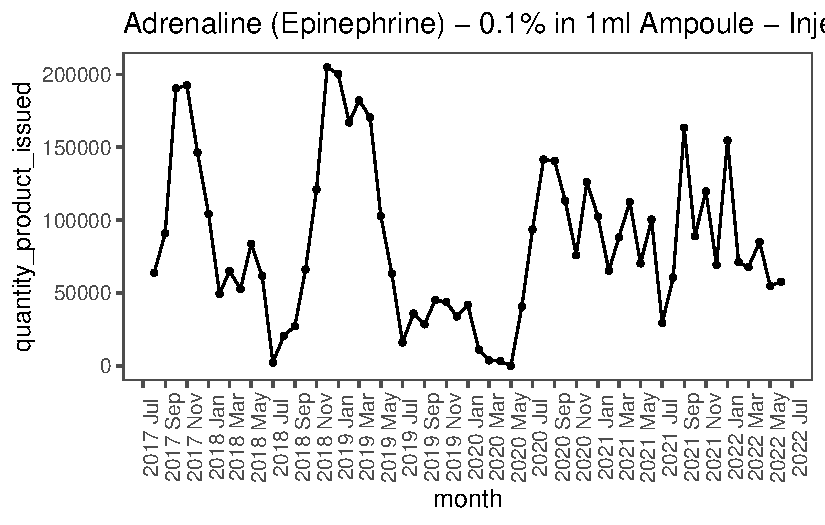
\includegraphics{main_files/figure-pdf/unnamed-chunk-10-1.pdf}

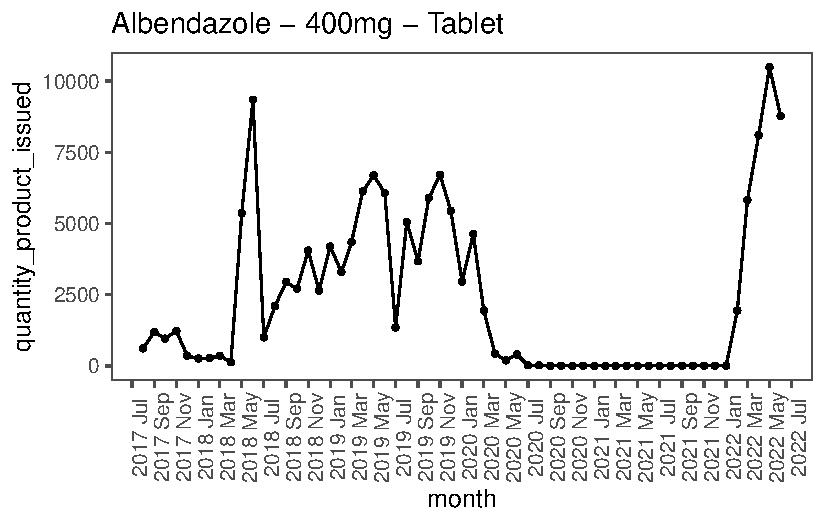
\includegraphics{main_files/figure-pdf/unnamed-chunk-11-1.pdf}

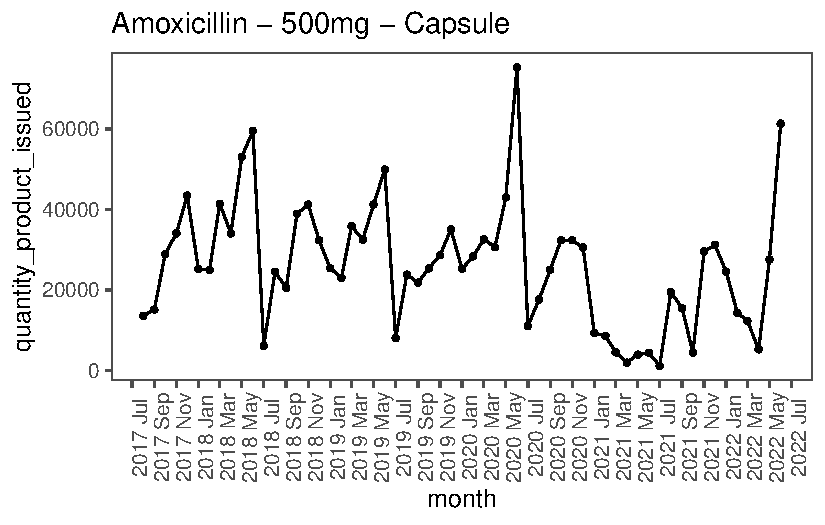
\includegraphics{main_files/figure-pdf/unnamed-chunk-12-1.pdf}

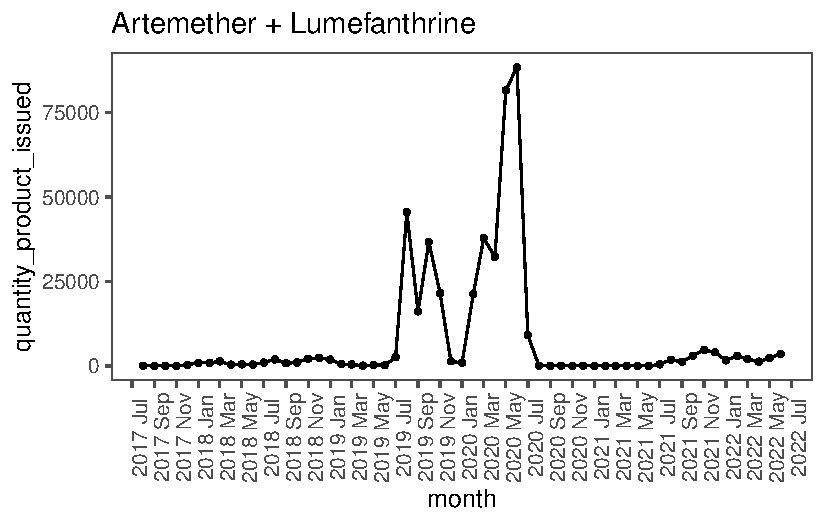
\includegraphics{main_files/figure-pdf/unnamed-chunk-13-1.pdf}

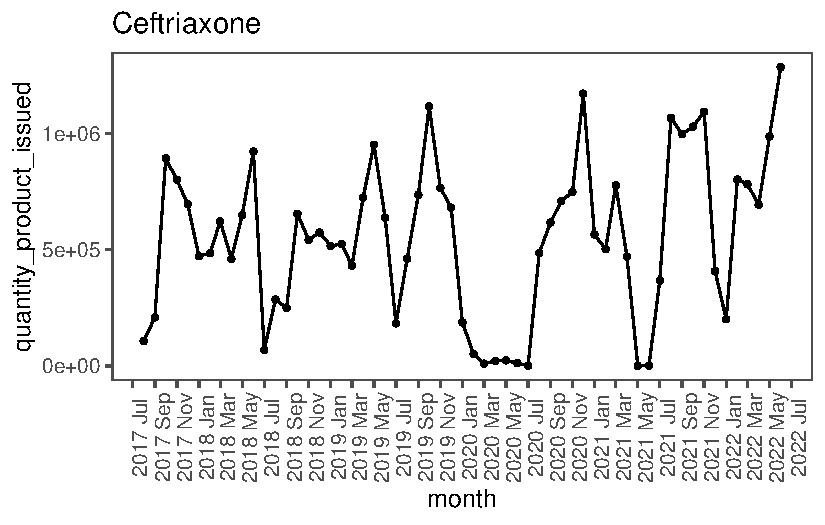
\includegraphics{main_files/figure-pdf/unnamed-chunk-14-1.pdf}

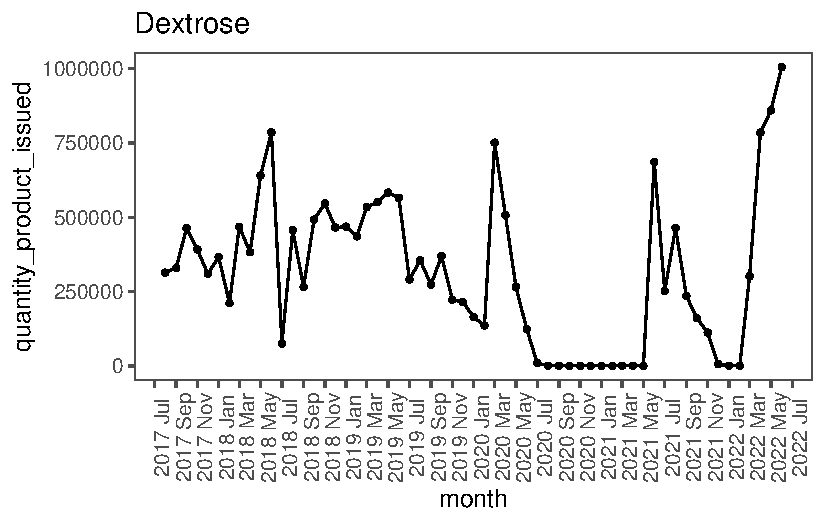
\includegraphics{main_files/figure-pdf/unnamed-chunk-15-1.pdf}

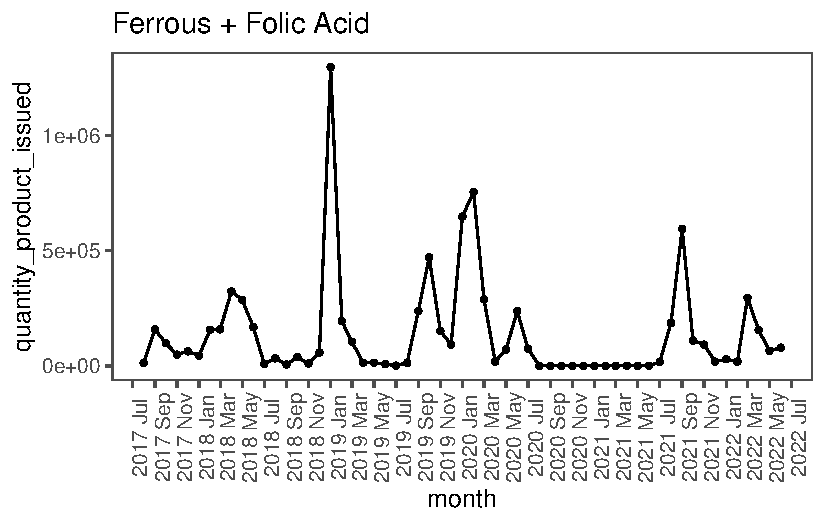
\includegraphics{main_files/figure-pdf/unnamed-chunk-16-1.pdf}

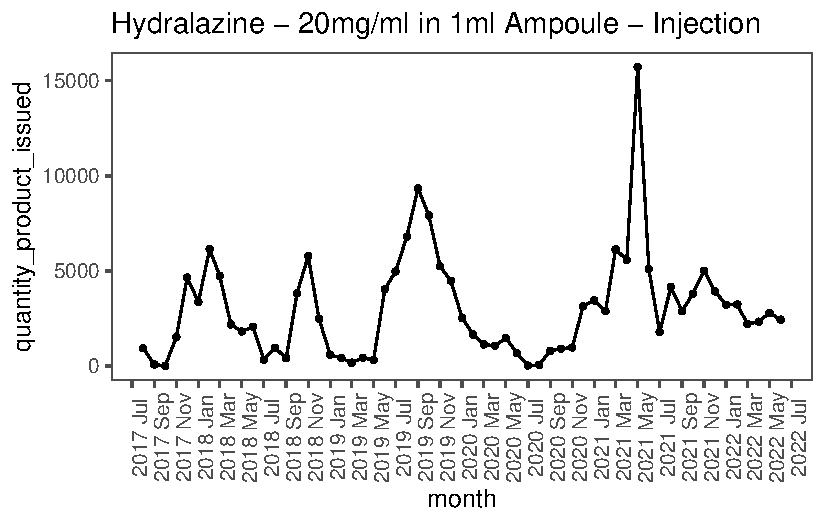
\includegraphics{main_files/figure-pdf/unnamed-chunk-17-1.pdf}

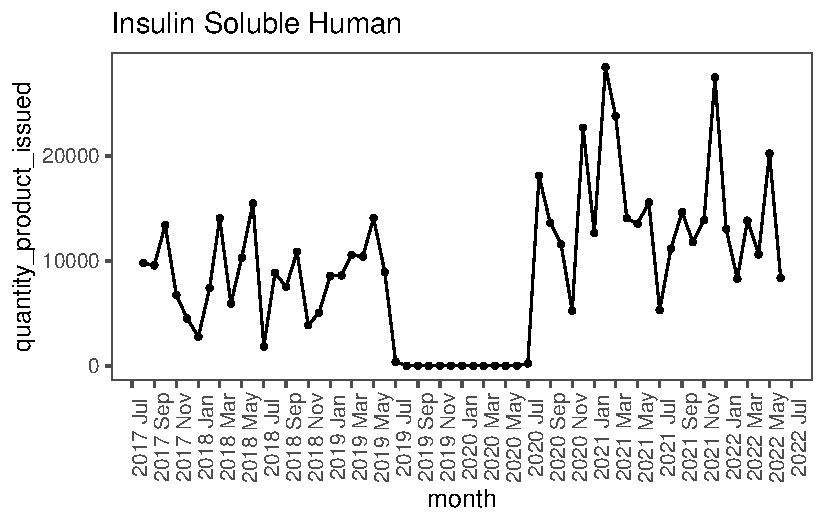
\includegraphics{main_files/figure-pdf/unnamed-chunk-18-1.pdf}

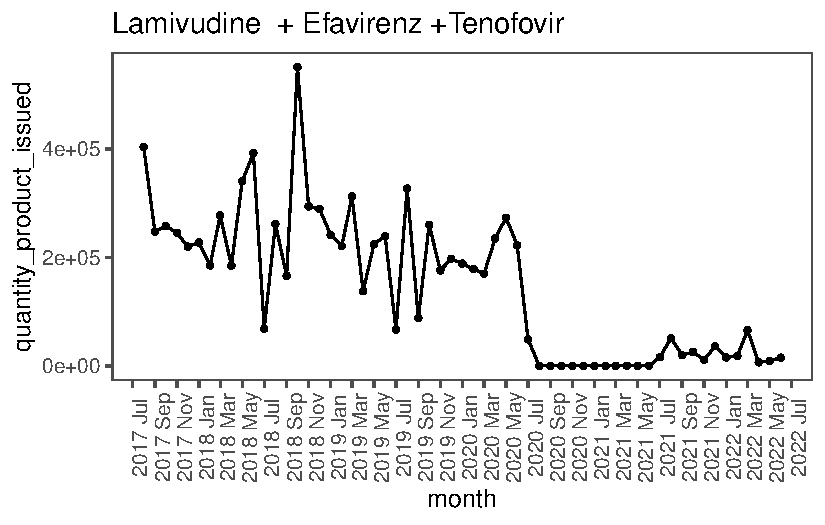
\includegraphics{main_files/figure-pdf/unnamed-chunk-19-1.pdf}

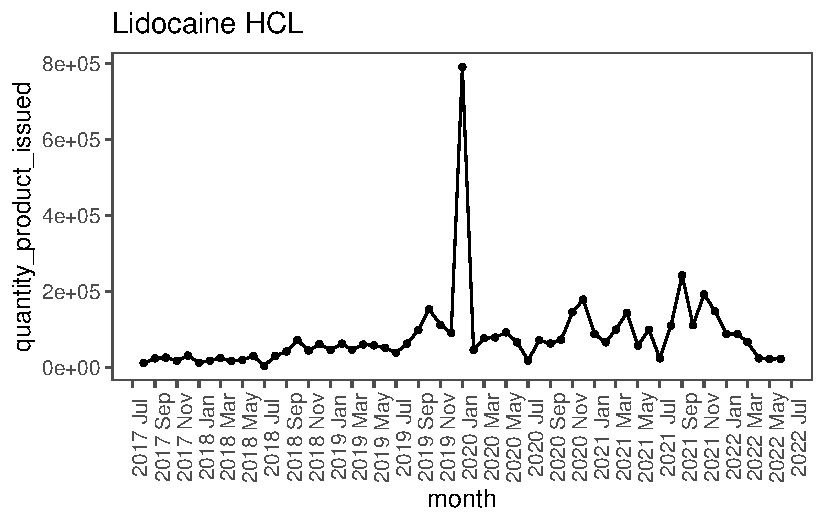
\includegraphics{main_files/figure-pdf/unnamed-chunk-20-1.pdf}

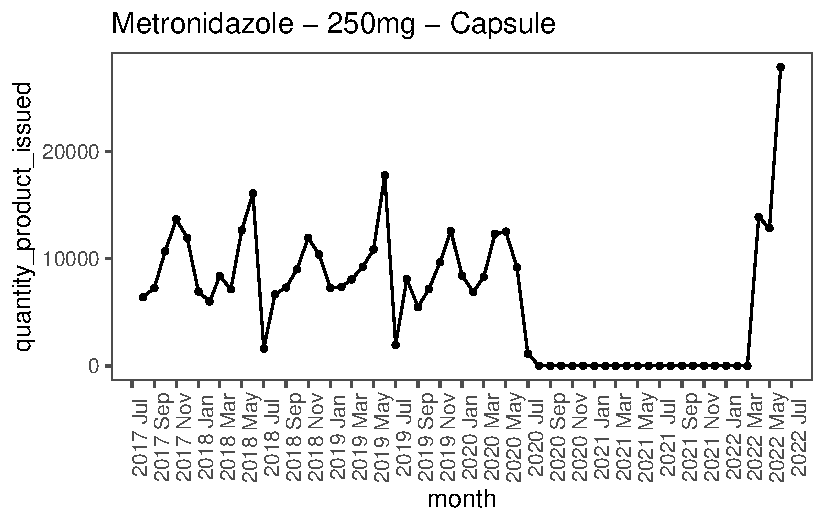
\includegraphics{main_files/figure-pdf/unnamed-chunk-21-1.pdf}

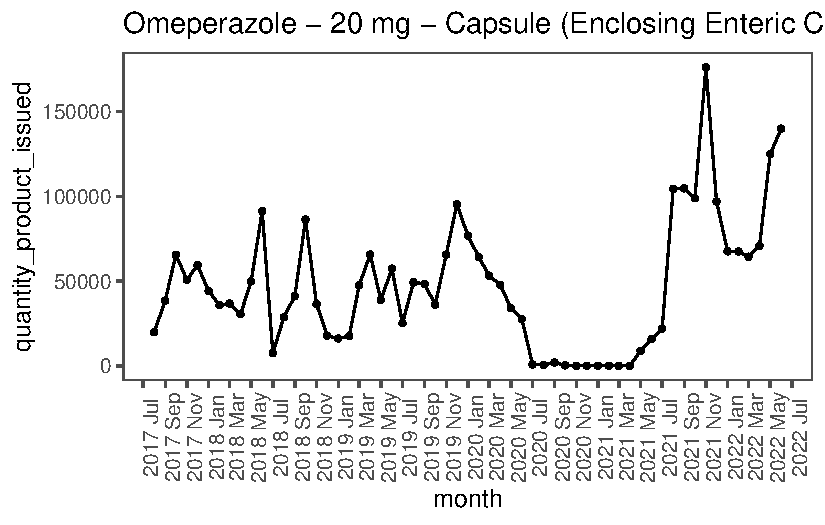
\includegraphics{main_files/figure-pdf/unnamed-chunk-22-1.pdf}

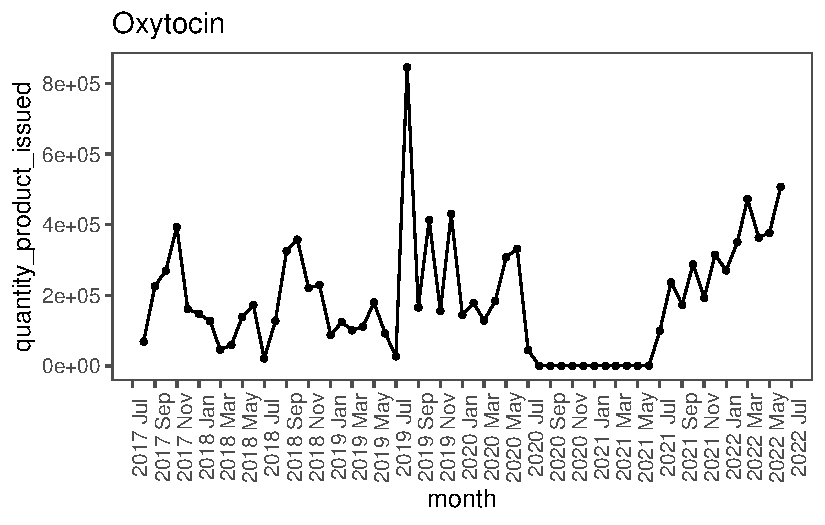
\includegraphics{main_files/figure-pdf/unnamed-chunk-23-1.pdf}

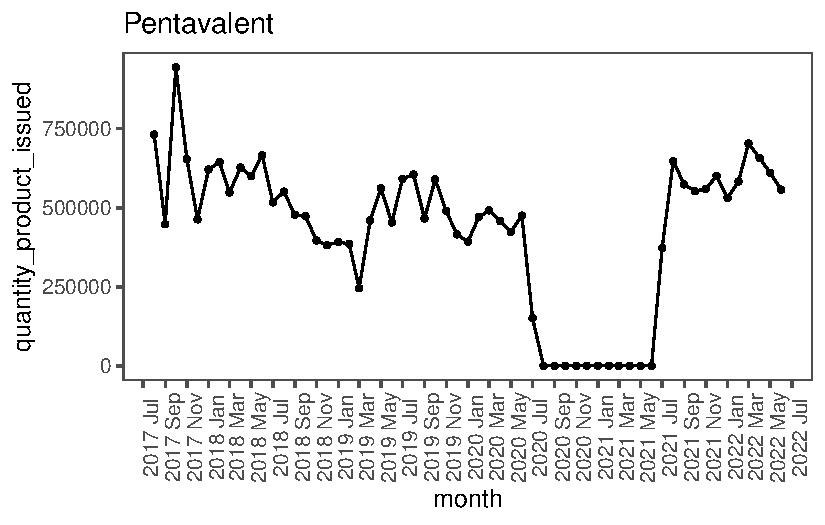
\includegraphics{main_files/figure-pdf/unnamed-chunk-24-1.pdf}

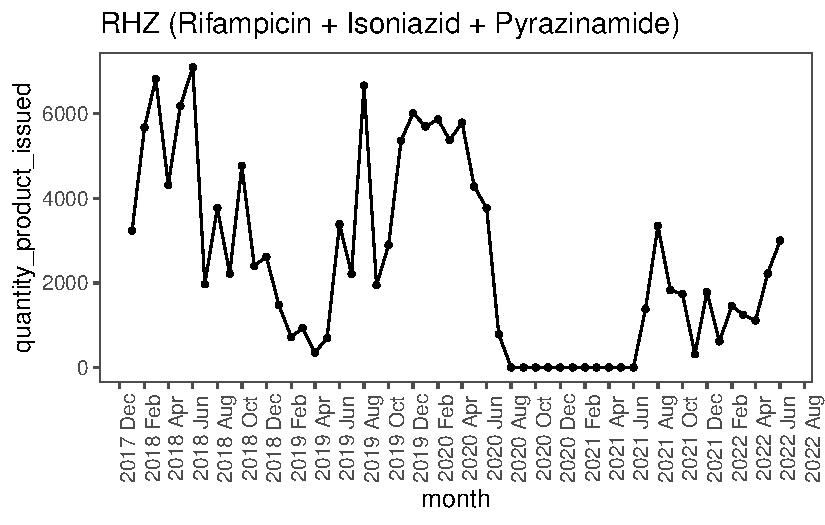
\includegraphics{main_files/figure-pdf/unnamed-chunk-25-1.pdf}

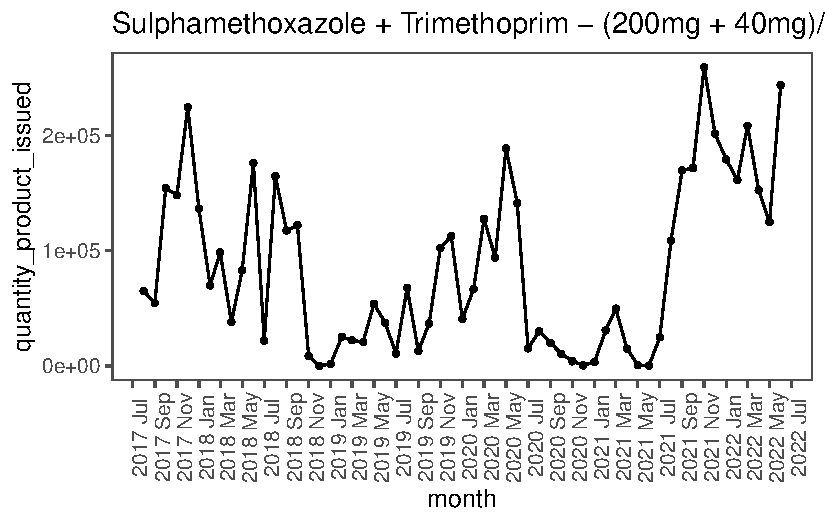
\includegraphics{main_files/figure-pdf/unnamed-chunk-26-1.pdf}

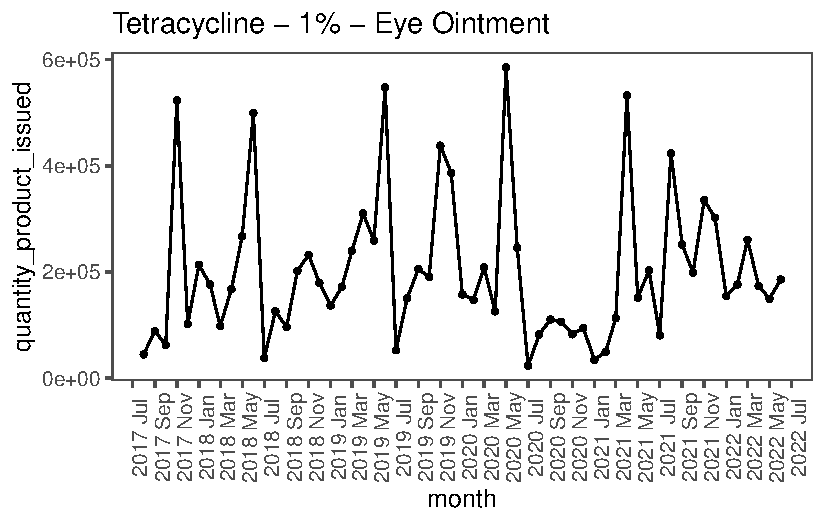
\includegraphics{main_files/figure-pdf/unnamed-chunk-27-1.pdf}

\hypertarget{data-splitting-and-preparation}{%
\section{2. 2. Data Splitting and
Preparation}\label{data-splitting-and-preparation}}

The primary objective of this study is to forecast pharmaceutical demand
within EPSS for the year 2023. To achieve this, the historical sales
data for the chosen pharmaceuticals in EPSS was partitioned into
distinct training and testing subsets. Employing the widely recognized
70:30 split method, 70\% of the available data was designated as the
training set, while the remaining 30\% was reserved for testing and
validation purposes \citep{chan2019comparison}. As a result, the dataset
was segregated into a training set consisting of 42 months and a testing
set spanning 18 months

\hypertarget{forecasting-methods}{%
\section{2.3.1. Forecasting Methods}\label{forecasting-methods}}

In pursuit of accurate pharmaceutical demand forecasts, we explored a
spectrum of forecasting techniques. The following methods were applied:

Naive Method: A simple approach relying on the assumption that the
future value will be the same as the most recent observed value.This
Methods uses when there is no seasonality
\citetext{\citealp[burinskiene2022forecasting]{article}; \citealp[nikolopoulos2016forecasting]{article}}
Mean Method: A straightforward technique forecasting future values based
on the mean of past observations. Seasonal Naive Method: Similar to the
naive method, this approach predicts future values using the most recent
observed value from the same season. Exponential Smoothing: A method
that assigns exponentially decreasing weights to past observations to
forecast future values. Regression: Employing statistical regression
models to establish relationships between variables for prediction.
Autoregressive Integrated Moving Average Model (ARIMA): A time series
model incorporating autoregressive, differencing, and moving average
components for accurate forecasting. ARIMA with Predictors: Extending
the ARIMA model with additional predictor variables to enhance
forecasting accuracy. Combination of Models: Exploring ensemble methods
that combine multiple models for improved predictive performance. By
applying these diverse forecasting methodologies, we aimed to
comprehensively assess and compare their efficacy in predicting
pharmaceutical demand within EPSS. Each method was evaluated against the
testing dataset to ascertain its forecasting accuracy and suitability
for the specific

\hypertarget{sec-method}{%
\subsection{Forecasting methods}\label{sec-method}}

Model building

\hypertarget{naive}{%
\section{Naive}\label{naive}}

The naive forecast method is a simple approach that assumes future
values will be the same as the most recent observed value, making it
useful for stable or slowly changing time series. While it doesn't
consider underlying patterns, it serves as a baseline for evaluating
more advanced techniques\citep{hyndman2018forecasting}. It's
particularly suitable for products with stable demand or limited
seasonality, providing a straightforward reference for forecasting and
inventory management.

\hypertarget{mean}{%
\section{Mean}\label{mean}}

The mean forecast method predicts future values by averaging historical
data, making it suitable for stable time series. While it overlooks
trends and seasonality, it serves as a baseline for evaluating advanced
techniques \citep{hyndman2018forecasting}. Its simplicity makes it
valuable in certain forecasting applications
\citep{hyndman2018forecasting}.

\hypertarget{seasonal-naive}{%
\section{Seasonal naive}\label{seasonal-naive}}

The seasonal naive forecast method predicts future values based on the
most recent observed value from the corresponding season in the previous
year, making it useful for data with strong seasonal patterns. It serves
as a baseline for evaluating seasonal forecasting models, capturing
repetitive patterns effectively. Its simplicity and ability to capture
seasonality make it valuable in seasonal forecasting
applications\citep{hyndman2018forecasting}.

\hypertarget{exponential-smoothing}{%
\section{Exponential smoothing}\label{exponential-smoothing}}

Exponential Smoothing is regarded as one of the most accurate and robust
methods for time series forecasting. Not only does it exhibit high
accuracy, but it also offers versatility and robustness. What makes
Exponential Smoothing particularly appealing is its intuitive nature,
making it easy to understand and interpret. Furthermore, this method
boasts minimal data storage and computational requirements, making it
highly efficient for real-time applications. In the business realm,
Exponential Smoothing finds extensive use for inventory demand
forecasting, showcasing its practicality \citep{gardner1985exponential}.
Surprisingly, even when pitted against more sophisticated techniques,
Exponential Smoothing has demonstrated impressive performance in
forecasting competitions
\citep[\citet{makridakis1982accuracy}]{makridakis2000m3}. Its simplicity
and reliability make it a widely trusted approach in the field of
forecasting.

\hypertarget{regression}{%
\section{Regression}\label{regression}}

Regression methods play a crucial role in forecasting and optimizing the
health supply chain, ensuring the availability and efficient
distribution of essential medical resources. By analyzing historical
data, regression models can identify patterns and relationships between
variables such as patient demand, disease prevalence, and inventory
levels. The basic concept is that we forecast the time series of
interest assuming that it has a linear relationship with other time
series. For example, we might wish to forecast monthly sales y using
total advertising spend as a predictor X. Or we might forecast daily
electricity y demand using temperature x1 and the day of week x2 as
predictors. The forecast variable y is sometimes also called the regress
and, dependent or explained variable. The predictor variables x are
sometimes also called the regressors, independent or explanatory
variables.

Simple linear regression In the simplest case, the regression model
allows for a linear relationship between the forecast variable y and a
single predictor variable x: yt = β0 + β1xt + ε Example of data from
such a model is shown in Figure 5.1. The coefficients β0 and β1 denote
the intercept and the slope of the line respectively. The intercept β0
represents the predicted value of y when x=0 . The slope represents the
average predicted change in y resulting from a one unit increase in x.

\hypertarget{figure-an-example-of-data-from-a-simple-linear-regression-model}{%
\section{Figure : An example of data from a simple linear regression
model}\label{figure-an-example-of-data-from-a-simple-linear-regression-model}}

Notice that the observations do not lie on the straight line but are
scattered around it. We can think of each observation yt as consisting
of the systematic or explained part of the model, = β0 + β1xt , and the
random ``error'', εt. The ``error'' term does not imply a mistake, but a
deviation from the underlying straight line model. It captures anything
that may affect yt other than xt

Multiple linear regressions When there are two or more predictor
variables, the model is called a multiple regression model. The general
form of a multiple regression model is

yt = β0 + β1x1,t + β2x2,t + ⋯ + βkxk,t + εt, (1)

where is the variable to be forecast and are the predictor variables.
Each of the predictor variables must be numerical. The coefficients
β1,\ldots.. βk measure the effect of each predictor after taking into
account the effects of all the other predictors in the model. Thus, the
coefficients measure the marginal effects of the predictor variables.
Assumptions When we use a linear regression model, we are implicitly
making some assumptions about the variables in Equation (1).

First, we assume that the model is a reasonable approximation to
reality; that is, the relationship between the forecast variable and the
predictor variables satisfies this linear equation.

Second, we make the following assumptions about the errors (ε1, \ldots{}
, εT ) :

they have mean zero; otherwise the forecasts will be systematically
biased.

they are not autocorrelated; otherwise the forecasts will be
inefficient, as

there is more information in the data that can be exploited.

they are unrelated to the predictor variables; otherwise there would be
more information that should be included in the systematic part of the
model.

It is also useful to have the errors being normally distributed with a
constant variance σ2 in order to easily produce prediction intervals.
Another important assumption in the linear regression model is that each
predictor x is not a random variable. If we were performing a controlled
experiment in a laboratory, we could control the values of each x (so
they would not be random) and observe the resulting values of y. With
observational data (including most data in business and economics), it
is not possible to control the value of x, we simply observe it. Hence
we make this an assumption.

\hypertarget{auto-regressive-integrated-moving-average-model-arima}{%
\section{Auto regressive Integrated Moving Average Model
(ARIMA)}\label{auto-regressive-integrated-moving-average-model-arima}}

The Autoregressive Integrated Moving Average (ARIMA) model is a widely
utilized approach for forecasting and analyzing time series data. It
combines three key components: autoregression (AR), differencing (I),
and moving average (MA). ARIMA models have been extensively studied and
applied in various domains due to their flexibility and effectiveness in
capturing both short-term and long-term dependencies in time series.Box
and Jenkins (1970) {[}1{]} introduced the ARIMA model as a powerful tool
for time series analysis. The authors provided a comprehensive framework
for identifying, estimating, and diagnosing ARIMA models. They
emphasized the importance of differencing to achieve stationarity in
non-stationary time series data, allowing the model to capture trends
and patterns effectively.

\citep{chase2013demand} describes the application of the ARIMA model. It
is the forecasting technique that integrates vital components of
time-series and methods of regression. In 1970, George Box and Gwilym
Jenkins introduced the ARIMA forecasting method, and they developed a
comprehensive approach for forecasting \citep{chase2013demand}.ARIMA
(p,d,q) models gather relevant factors from the historical data by using
auto-correlation between them to distinguish those slacked request
verifiable qualities that best anticipate future demand; whereas p is
the order of Autoregressive (AR) term, q is the order of MA term

ARIMA can demonstrate cycle and regularity, and is mainly used for
mid-term aggregate forecasts and pre-sent far superior estimations than
time series models or even casual models; explained by
\citep{stadtler2014supply} explicitly considers dependent demands.
Additionally, different components, for example, informative factors
that impact request. It is also considered a good fit for the Mean
Absolute Percentage Errors (MAPE) calculation.

ARIMA model helps analyse the time series's probabilistic properties and
develop sin-gle or multi-equation models \citep{moritz2015comparison}.
Analysing a time series data is that there is a straightforward yet
extensive arrangement of useful models that can speak to numerous
conceivable examples of information found in time series. For a
stationary time-series, we can envision the information creating process
as a weighted blend of earlier perceptions in addition to an irregular
request term. Besides, identifying the ARIMA model parameters (i.e.~p, q
and d) is often challenging. Thereby, we use R software's statistical
package; it is widely used in the relevant literature
\citep{bokde2016psf, dhamo2010using}. Moreover, `R' generated the best
combination of p, d and q values because it estimates the value of the
parameter based on AIC (Akaike Information Criterion) and BIC (Bayesian
Information Criterion).

\#Performance evaluation \{\#sec-performance\}

\hypertarget{forecast-accuracy-measures}{%
\section{2.4. Forecast accuracy
measures}\label{forecast-accuracy-measures}}

To evaluate the forecast accuracy and bias, several measures including
Root Mean Squared Error (RMSE), Mean Absolute Error (MAE), Mean Absolute
Scaled Error (MASE), Root Mean Squared Scaled Error (RMSSE),and Winkler
are used. We only present the results for RMSSE due to the space limit
of the journal and also because it is the recommended error metric in M5
competition \citep{makridakis2022m5}.

Point forecast accuracy is measured via the Mean Squared Scaled Error
(MSSE) and the Mean Absolute Scaled Error (MASE). The Mean Absolute
Scaled Error (MASE)
\citep[hyndman2018forecasting,\citet{article}hyndman2006another,]{book}
is calculated as ::: \{.cell
hash=`main\_cache/pdf/unnamed-chunk-28\_a96c898b6cc2c723121cc3be6c515a81'\}

:::

\hypertarget{sec-results}{%
\section{Results and discussion}\label{sec-results}}

from the total of 37 key pharmaceuticals selected and tested with the
different forecasting models arima showed that a better forecast
accuracy for most of the pharmaceuticals followed by mean and
regresstion models with RMSSE value of 0.850, 0.942 and 0.945
respectively (Table 1).

\begin{table}[!h]
\centering
\begin{tabular}[t]{lrrrrrr}
\toprule
.model & RMSE & MAE & MASE & RMSSE & winkler & CRPS\\
\midrule
arima & 109214.1 & 91630.74 & 0.925905 & 0.8503067 & 683471.4 & 64771.83\\
exponential_smoothing & 117985.6 & 98588.74 & 1.048426 & 0.9579627 & 695575.3 & 68638.44\\
mean & 121312.5 & 107616.64 & 1.087621 & 0.9422224 & 582790.3 & 73334.54\\
naive & 135300.5 & 116398.62 & 1.268535 & 1.0841642 & 570090.5 & 74691.10\\
regression & 131416.4 & 114329.68 & 1.065268 & 0.9455063 & 899543.3 & 83315.32\\
\addlinespace
snaive & 143861.2 & 122377.80 & 1.165142 & 1.0463095 & 732046.7 & 85266.80\\
\bottomrule
\end{tabular}
\end{table}

Then we tested the models by adding different predictors which affects
the sales of the pharmaceuticals like physical count, budget release and
budget closure by the government, COVID 19, campaign in to the models as
predictors which will affects the sales of the key pharmaceuticals
products and the result showed that still arima have a better forecast
accuracy with RMSSE of 0.850 (Table 2).

\begin{table}[!h]
\caption{forecast accuarcy of selected pharmaceuticals in EPSS 2018-2022 after
considering predictors}\tabularnewline

\centering
\begin{tabular}[t]{lrrrrrr}
\toprule
.model & RMSE & MAE & MASE & RMSSE & winkler & CRPS\\
\midrule
arima_predictor & 114064.7 & 95753.88 & 0.9192677 & 0.851753 & 807586.4 & 68631.70\\
regression_predictor & 132117.6 & 113194.12 & 1.0474410 & 0.941347 & 1000434.4 & 83390.61\\
\bottomrule
\end{tabular}
\end{table}

\begin{figure}

{\centering 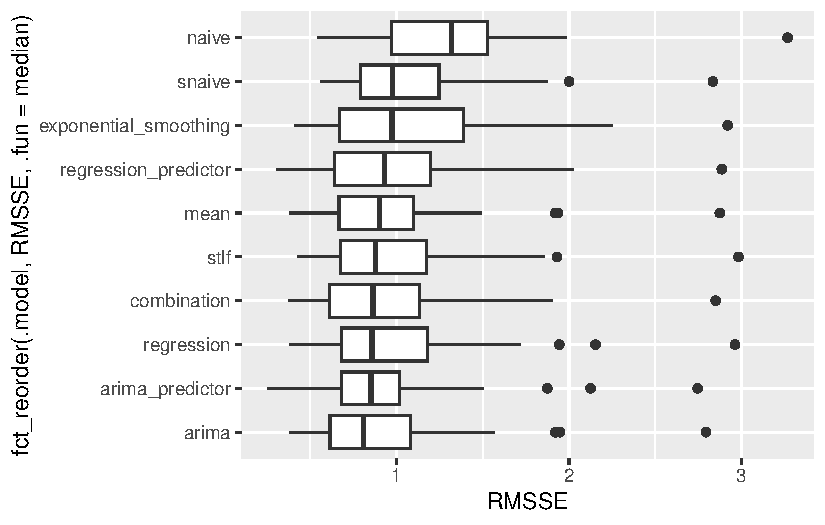
\includegraphics{main_files/figure-pdf/result2-1.pdf}

}

\caption{forecast accuarcy of selected pharmaceuticals in EPSS 2018-2022
after considering predictors}

\end{figure}

Individual item with different forecasting models We tested 10 models
namely arima, arima with predictor, combination, exponential smoothing,
mean, naive, regression, regression with predictor, snaive and stlf.
Individually on the selected key pharmaceuticals and the result
indicated that 11 (32.43\%) of the selected pharmaceuticals have better
forecast accuracy for arima predictor models, followed by naive 6
(16.21\%), mean, regresstion, arima, and STLF methods each of them with
3 (8.10\%) (Fig 2)

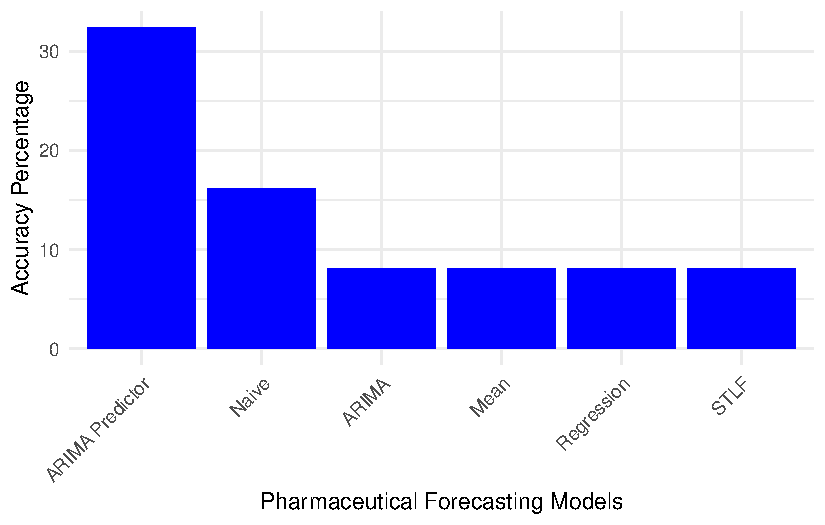
\includegraphics{main_files/figure-pdf/unnamed-chunk-43-1.pdf}

Those pharmaceuticals who had a better forecast accuracy with Arima
predictors are Amoxacillin 500mg capsule, Anti RhD, Artehmether +
Lumefantrine, Atenolol, Atrovastatin 200mg, Ferrosu sulphate with follic
acid, frusemide injection, Insuline Iosphane bipahsic, Lamivudine
+Efaverienze + Tenofovir, Lidocaine + HCL and Propyl thiro uracil.The
six pharmaceuticasl which showed a better forecast accuracy with naive
models were Ciprofloxacillin 500mg tablet, Magnesoum sulphate injection,
Omeprazole capsule, Omeprazole injection, Rapid diagnostic test,
Sulphamethaxone + Trimetoprine tablet.

Discussion:

The objective of this study was to evaluate the forecasting accuracy of
different models for key selected pharmaceutical products from the
Ethiopian Pharmaceutical Supply Services (EPSS). The analysis
encompassed a total of 37 key pharmaceutical products, and the results
highlight the performance of various forecasting models in predicting
sales for these products. In the initial assessment of forecasting
models, the ARIMA model emerged as the most accurate for the majority of
the pharmaceutical products, exhibiting a Root Mean Squared Scaled Error
(RMSSE) value of 0.850. This finding suggests that ARIMA has a strong
predictive capability and outperforms other models, including the mean
and regression models. The superiority of the ARIMA models over the
Moving Average might be explained by most of the data set have seasonal
patern and MA is one of the simplest prediction techniques for making
projections about time-series without a noticeable seasonal pattern
\citep{chopra2001supply}.The superiority of the ARIMA model underscores
its suitability for pharmaceutical sales forecasting within the context
of EPSS. Similar findings were reported in forecasting ethanol demand in
India where ARIMA model outperforms other models like linear and
non-linear regression models \citep{dey2023forecasting}.

To enhance the predictive power of the models, additional predictors
were incorporated into the analysis. Predictors such as physical count,
budget release and closure by the government, the impact of COVID-19,
and promotional campaigns were considered as potential drivers of
pharmaceutical sales. Despite the inclusion of these predictors, the
ARIMA model maintained its superior forecasting accuracy with an RMSSE
of 0.850. This resilience further validates the robustness of the ARIMA
model and its ability to capture complex interactions between variables
influencing pharmaceutical sales.

To delve deeper into the individual performance of the forecasting
models, a comprehensive evaluation was conducted on each of the 37
pharmaceutical products. Among the ten models tested, ARIMA with
predictors exhibited the highest forecast accuracy for 32.43\% of the
products. This was followed by the naive model, which performed well for
16.21\% of the products. Notably, a few pharmaceuticals demonstrated a
strong fit with specific models. For instance, Amoxicillin 500mg
capsule, Anti RhD, Artehmether + Lumefantrine, and others exhibited
superior forecast accuracy when utilizing the ARIMA model with
predictors.

Similarly, other pharmaceuticals displayed better forecasting outcomes
with alternative models. Notably, Ciprofloxacin 500mg tablet, Magnesium
sulfate injection, Omeprazole capsule, and others showed improved
accuracy with the naive model. These findings underscore the importance
of tailoring the choice of forecasting model based on the
characteristics and dynamics of individual pharmaceutical products.This
finding confirmed that There is not a single best technique to solve
time-series forecasting problems \citep{zhang2007quarterly}. In order to
deal with time-series forecasting, each problem might be solved with a
different approach \citep{ensafi2022time}.

In conclusion, this study highlights the pivotal role of accurate
forecasting in the pharmaceutical supply chain management. The ARIMA
model, particularly when integrated with relevant predictors, emerges as
a powerful tool for predicting pharmaceutical sales within the EPSS.
However, the selection of the most appropriate model should consider the
specific attributes of each pharmaceutical product. Further research
could explore the optimization of model parameters and the incorporation
of additional contextual variables to enhance forecasting accuracy and
supply chain efficiency.

Limitation

One notable limitation of this study revolves around the availability
and quality of the data used for analysis. While we employed a
comprehensive dataset from the EPSS, it is essential to acknowledge that
the accuracy of forecasting models is heavily contingent on the quality,
granularity, and completeness of historical sales data. Variations in
data recording practices, potential errors, missing values, or
inconsistencies within the dataset could impact the precision of the
forecasts generated by the employed models. Moreover, the inherent
complexity of pharmaceutical demand, influenced by a myriad of external
factors such as socioeconomic changes,stock outs, prolonged procurement
lead time, rationing of avaiable products, pushing of pharmaceuticals to
different health facility without demand, healthcare policies, and
unforeseen events, may introduce an additional layer of uncertainty. It
is important to recognize that despite our best efforts to address
data-related challenges, the robustness and reliability of our
forecasting outcomes may still be subject to the limitations inherent in
the original data.

\hypertarget{sec-conclusion}{%
\section{Conclusion}\label{sec-conclusion}}

In this study, we embarked on a comprehensive analysis of pharmaceutical
demand forecasting within the Ethiopian Pharmaceutical Supply Services
(EPSS) context. By leveraging five years of sales data for 37 key
pharmaceutical products, we aimed to enhance the accuracy of demand
predictions and consequently contribute to more effective supply chain
management. Our findings underscore the significance of accurate demand
forecasting in optimizing inventory levels, resource allocation, and
overall supply chain operations.

The application of diverse forecasting models yielded valuable insights
into their respective performance. Notably, the Autoregressive
Integrated Moving Average (ARIMA) model emerged as a robust choice,
consistently exhibiting superior forecast accuracy across a majority of
the selected pharmaceutical products. Additionally, the incorporation of
predictor variables, such as physical count, budget release and closure
by the government, COVID-19 impact, and campaign events, further
underscored the efficacy of the ARIMA model in accommodating external
influences and delivering reliable forecasts.

The individualized assessment of forecasting models revealed specific
strengths across pharmaceutical categories. ARIMA models with predictors
demonstrated exceptional performance for pharmaceuticals including
Amoxacillin 500mg capsule, Anti RhD, Artehmether + Lumefantrine,
Atenolol, and others, affirming their utility in capturing complex
demand patterns. Moreover, the study shed light on pharmaceuticals best
suited for alternative models like naive, mean, and regression methods,
contributing to a comprehensive understanding of forecasting
applicability.

While these findings contribute significantly to the discourse on
pharmaceutical demand forecasting, it's essential to acknowledge
limitations. The accuracy of our forecasts is intrinsically linked to
the quality and completeness of historical sales data, and the intricate
interplay of external variables adds complexity to the forecasting
landscape.

In conclusion, this study serves as a pivotal step towards enhancing
pharmaceutical supply chain management through refined demand
forecasting. The demonstrated success of ARIMA models, particularly when
augmented with predictor variables, holds promise for fostering
resilient and adaptable supply chains. As the pharmaceutical landscape
continues to evolve, our insights encourage further exploration of
advanced forecasting techniques and continuous refinement of strategies
to bolster supply chain efficiency and ensure consistent availability of
essential pharmaceuticals.

In light of the study's findings, several actionable recommendations
emerge. First and foremost, the integration of the Autoregressive
Integrated Moving Average (ARIMA) model with predictor variables stands
out as a viable strategy for enhancing pharmaceutical demand forecasting
accuracy within Ethiopian Pharmaceutical Supply Services (EPSS). This
entails harnessing the predictive power of external factors to refine
forecasting precision. To further advance forecasting practices, the
exploration of additional predictor variables such as public health
campaigns, disease outbreaks, and economic indicators could offer
valuable insights into demand dynamics. Moreover, refining the
granularity of historical sales data, possibly through finer temporal
intervals and geographic diversity, holds potential for more nuanced and
accurate predictions. Consideration could also be given to hybrid
forecasting models that amalgamate ARIMA's short-term accuracy with
machine learning's predictive prowess for long-term trends. Regular
model evaluation, sensitivity analysis, and collaborative stakeholder
engagement are recommended to ensure ongoing accuracy and alignment with
changing demand patterns.

Capacitating EPSS staff through training programs in forecasting
methodologies and data interpretation can empower the workforce to make
informed decisions. Replication of this study in diverse healthcare
settings and comparative analyses can validate the findings'
applicability and adaptability. By embracing these recommendations, EPSS
can fortify its pharmaceutical supply chain with resilient, efficient,
and responsive operations, ultimately ensuring the consistent
availability of vital pharmaceuticals. a

\hypertarget{reproducibility}{%
\section*{Reproducibility}\label{reproducibility}}
\addcontentsline{toc}{section}{Reproducibility}

R code to produce all results in this paper is available at


\renewcommand\refname{References}
  \bibliography{references.bib}


\end{document}
